%% LyX 2.2.1 created this file.  For more info, see http://www.lyx.org/.
%% Do not edit unless you really know what you are doing.
\documentclass[12pt,english]{article}
\usepackage[T1]{fontenc}
\usepackage[latin9]{inputenc}
\usepackage[a4paper]{geometry}
\geometry{verbose,tmargin=1cm,bmargin=1cm,lmargin=1cm,rmargin=1cm}
\usepackage{amsmath}

\makeatletter

%%%%%%%%%%%%%%%%%%%%%%%%%%%%%% LyX specific LaTeX commands.
%% Because html converters don't know tabularnewline
\providecommand{\tabularnewline}{\\}

%%%%%%%%%%%%%%%%%%%%%%%%%%%%%% User specified LaTeX commands.
\usepackage{pgf}
\usepackage{tikz}
\usetikzlibrary{arrows,automata}

\makeatother

\usepackage{babel}
\begin{document}

\title{Reinforcement learning ( CS6700 )\\
Written assignment \#3}

\author{Aravind S\\
EE14B013}

\date{13th Mar. 2017}
\maketitle

\section{Problem 1}

No discounting here. Easy!

\subsection{Part (a)}

Monte-Carlo estimates are average of rewards observed from a particular
state ( from all episodes ) till termination. Multiple visits to a
state are ignored as we are doing first-visit Monte-Carlo.\\
\\
For state $B$,\\
\\
\begin{alignat*}{1}
V(B) & =\frac{(1)+(0+2)+(0+0+1)+(0+2)+(0+0+1)+(0+2)+(1)+(1)+(1)+(1)}{10}=1.30
\end{alignat*}
\\
\\
For state $A$,\\
\\
\begin{alignat*}{1}
V(A) & =\frac{(0+1)+(2)+(0+0+2)+(0+0+0+1)+(2)+(0+1)+(2)+(0+1)}{8}=1.50
\end{alignat*}


\subsection{Part (b)}

Based on possible transitions we can obtain an estimate of transition
probabilities. The possible transitions here include $A\rightarrow B$,
$A\rightarrow T$, $B\rightarrow A$ and $B\rightarrow T$ where $T$
is a terminal state. We can build a transition matrix from the episodes.

\begin{tabular}{|c|c|c|c|}
\hline 
 & $A$ & $B$ & $T$\tabularnewline
\hline 
\hline 
$A$ & $0$ & $6$ & $4$\tabularnewline
\hline 
$B$ & $5$ & $0$ & $7$\tabularnewline
\hline 
$T$ & $0$ & $0$ & $0$\tabularnewline
\hline 
\end{tabular}\\
\\
where $a_{ij}(i^{th}row,j^{th}column)$ denotes the number of transitions
from $i\rightarrow j$.\\
\\
Now, $p(s_{t+1}=j\,|\,s_{t}=i)=\frac{n(s_{t+1}=j\,|\,s_{t}=i)}{n(s_{t}=i)}$
where $n(...)$ denotes number of occurences of $(...)$ in the episodes.
Calculating this for all possible transitions we get,\\
\\
\begin{tabular}{|c|c|c|}
\hline 
Transition & Probability & Value\tabularnewline
\hline 
\hline 
$A\rightarrow B$ & $p(s_{t+1}=B\,|\,s_{t}=A)$ & $0.6000$\tabularnewline
\hline 
$A\rightarrow T$ & $p(s_{t+1}=T\,|\,s_{t}=A)$ & $0.4000$\tabularnewline
\hline 
$B\rightarrow A$ & $p(s_{t+1}=A\,|\,s_{t}=B)$ & $0.4167$\tabularnewline
\hline 
$B\rightarrow T$ & $p(s_{t+1}=T\,|\,s_{t}=B)$ & $0.5833$\tabularnewline
\hline 
\end{tabular}\\
\\
\\
We can build a transition matrix for rewards as shown below.\\
\\
\begin{tabular}{|c|c|c|c|}
\hline 
 & $A$ & $B$ & $T$\tabularnewline
\hline 
\hline 
$A$ & $0$ & $\frac{0+0+0+0+0+0+0}{7}=0$ & $\frac{2+2+2+2}{4}=2$\tabularnewline
\hline 
$B$ & $\frac{0+0+0+0+0}{5}=0$ & $0$ & $\frac{1+1+1+1+1+1+1}{7}=1$\tabularnewline
\hline 
$T$ & $0$ & $0$ & $0$\tabularnewline
\hline 
\end{tabular}\\
\\
where $R_{ij}(i^{th}row,j^{th}column)$ denotes the average reward
obtained for transition $i\rightarrow j$.\\
\\
The state-transition diagram is shown below.\\
\\
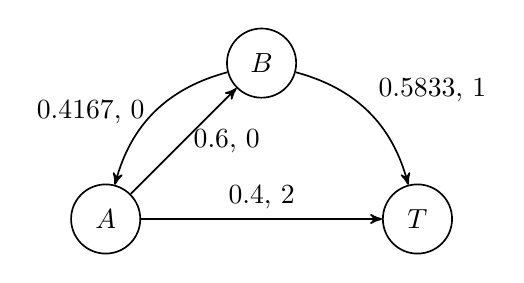
\begin{tikzpicture}[->,>=stealth',auto,node distance=2.8cm,semithick]
\tikzstyle{every state}=[text=black]
\node[state]         (A)					{$A$};
\node[state]         (B) [above right of=A] {$B$};
\node[state]         (T) [below right of=B] {$T$};


\path	(A) edge node		[right] {0.6, 0} (B)
		     edge		node {0.4, 2} (T)
		 (B) edge [bend right]		node[left] {0.4167, 0} (A)
		     edge [bend left]		node {0.5833, 1} (T);

\end{tikzpicture}		

\subsection{Part (c)}

Batch $TD(0)$ converges to the certainty-equivalence estimate for
the Markov model of the system. The Markov model is constructed based
on the given episodes only ( shown in part (b) ).\\
\\
$V(T)=0.$ Based on transition probabilities,\\
\\
$V(B)=0.5833(R(B,T)+V(T))+0.4167(R(B,A)+V(A))$\\
\\
$V(A)=0.4(R(A,T)+V(T))+0.6(R(A,B)+V(B))$\\
\\
Solving the above system of equations, we get,\\
\\
\begin{tabular}{|c|c|}
\hline 
State $s$ & Value $V(s)$\tabularnewline
\hline 
\hline 
$A$ & $1.5333$\tabularnewline
\hline 
$B$ & $1.2222$\tabularnewline
\hline 
$T$ & $0$\tabularnewline
\hline 
\end{tabular}

\section{Problem 2}

\subsection{Part (a)}

State-space $S=\{laughter\,(\,L\,),\,silent\,(\,S\,)\}$\\
\\
Actions $A=\{playing\,organ\,(O),\,lighting\,incense\,(I)\}$\\
\\
Discount factor $\gamma=0.9$.\\
\\
Let us consider the following way of action-encodings. We will assume
that if you burn incense, you won't play organ. And if you play organ,
you don't burn incense. It doesn't matter as far as we get the optimal
policy in the end. Also, encoding this way results in faster convergence
of iterative methods.\\
\\
The state transition diagram is given below.\\
\\
\begin{tikzpicture}[->,>=stealth',auto,node distance=6cm,semithick]
\tikzstyle{every state}=[text=black]
\node[state]         (L)					{$L$};
\node[state]         (S) [right of=A] {$S$};


\path	(L) edge [loop above] node {$I$, $-1$} (L)
		     edge node [right] {$O$, $+1$} (S)
		 (S) edge [loop below] node {$I$, $+1$} (S)
		     edge [bend right] node [left] {$O$, $-1$} (L);

\end{tikzpicture}		\\
\\


\subsection{Part (b)}

\subsubsection{Policy iteration}
\begin{itemize}
\item Let us assume an initial estimate of policy, $\pi_{0}=\{L:I,\,S:I\}$.
The symbols are defined in the previous part. Note that in vector
notation, the order is: $L,S$ ( for states ).
\item $p_{\pi_{0}}=\begin{array}{cc}
1 & 0\\
0 & 1
\end{array}$. $r_{\pi_{0}}=\begin{array}{c}
-1\\
+1
\end{array}$ $V_{\pi_{0}}=(I-\gamma p_{\pi_{0}})^{-1}r_{\pi_{0}}=\begin{array}{c}
-10\\
10
\end{array}$
\item Now, $\pi_{1}(L)=argmax_{a}\{O:\,1+0.9(10),I:-1+0.9(-10)\}=argmax_{a}\{O:10,I:-10\}=O$\\
$\pi_{1}(S)=argmax_{a}\{O:\,-1+0.9(-10),I:1+0.9(10)\}=argmax_{a}\{O:-10,I:10\}=I$\\
Therefore, $\pi_{1}=\{L:O,\,S:I\}$.
\item $p_{\pi_{1}}=\begin{array}{cc}
0 & 1\\
0 & 1
\end{array}$. $r_{\pi_{1}}=\begin{array}{c}
+1\\
+1
\end{array}$ $V_{\pi_{1}}=(I-\gamma p_{\pi_{1}})^{-1}r_{\pi_{1}}=\begin{array}{c}
10\\
10
\end{array}$
\item Now, $\pi_{2}(L)=argmax_{a}\{O:\,1+0.9(10),I:-1+0.9(10)\}=argmax_{a}\{O:10,I:8\}=O$\\
$\pi_{2}(S)=argmax_{a}\{O:\,-1+0.9(10),I:1+0.9(10)\}=argmax_{a}\{O:8,I:10\}=I$\\
Therefore, $\pi_{2}=\{L:O,\,S:I\}$.
\item $\pi_{1}=\pi_{2}.$ Thereforce, policy iteration converged to the
optimal policy $\pi^{*}=\{L:O,\,S:I\}.$
\item And optimal value function $V^{*}=V_{\pi_{1}}=\{L:10,S:10\}.$
\end{itemize}

\subsubsection{Value iteration}
\begin{itemize}
\item Let us assume an initial estimate of value function, $V_{0}=\{L:0,S:0\}.$
\item Now, $V_{1}(L)=max_{a}\{O:1+0.9(0),I:-1+0.9(0)\}=1$.\\
$V_{1}(S)=max_{a}\{O:-1+0.9(0),I:1+0.9(0)\}=1.$
\item $V_{2}(L)=max_{a}\{O:1+0.9(1),I:-1+0.9(1)\}=1.9$.\\
$V_{2}(S)=max_{a}\{O:-1+0.9(1),I:1+0.9(1)\}=1.9.$
\item $V_{3}(L)=max_{a}\{O:1+0.9(1.9),I:-1+0.9(1.9)\}=2.71$.\\
$V_{3}(S)=max_{a}\{O:-1+0.9(1.9),I:1+0.9(1.9)\}=2.71.$
\item $V_{4}(L)=max_{a}\{O:1+0.9(2.71),I:-1+0.9(2.71)\}=3.439$.\\
$V_{4}(S)=max_{a}\{O:-1+0.9(2.71),I:1+0.9(2.71)\}=3.439.$
\item Following the trend, we can observe that $V^{*}$converges to $\{L:10,S:10\}$
( sum of G.P with $a=1,r=0.9$ ).
\end{itemize}

\subsection{Part (c)}

Now we know that $V^{*}=\{L:10,S:10\}$. Knowing this, we can compute
$Q^{*}(s,a)$ with one-step look ahead at $V^{*}$.\\
\\
$Q^{*}(L,O)=1+0.9V^{*}(S)=10$\\
$Q^{*}(L,I)=-1+0.9V^{*}(S)=8$\\
$Q^{*}(S,O)=-1+0.9V^{*}(L)=8$\\
$Q^{*}(S,I)=1+0.9V^{*}(L)=10$

\subsection{Part (d)}

Advice to At Wits End is to follow the optimal policy as it ensures
that the house remains silent. Since currently laughing sound is heard,
At Wits End should play his organ and after that the house becomes
silent. Now, he should switch and light an incense. He should keep
doing this forever i.e he should keep burning incense and the house
will be silent :). Stay happy At Wits End!

\section{Problem 3}

If we consider the given grid-world, there are totally $6$ states
out of which $2$ are terminal states. From the remaining states,
we can take some actions as shown below.\\
\\
\begin{tabular}{|c|c|c|c|c|}
\hline 
~~~ & ~~~ & ~S~ & ~~~ & ~~~\tabularnewline
\hline 
\hline 
T2 & {*} & A & B & T1\tabularnewline
\hline 
\end{tabular}\\
\\
It is given that there is a reward of $+5$ units when $T2$ is reached,
$+10$ units when $T1$ is reached and any transition to $*$ results
in a reward of $a$ units. \\
\\
\begin{tabular}{|c|c|c|c|c|}
\hline 
~~~ & ~~~ & ~$\downarrow$~ & ~~~ & ~~~\tabularnewline
\hline 
\hline 
X & $\begin{array}{c}
\leftarrow\\
\rightarrow
\end{array}$ & $\begin{array}{c}
\leftarrow\\
\rightarrow
\end{array}$ & $\begin{array}{c}
\leftarrow\\
\rightarrow
\end{array}$ & X\tabularnewline
\hline 
\end{tabular}\\
\\
From state $A$, we won't take the ``up'' action because there is
no reward obtained in the process and the only possible action from
state $S$ is coming down again. So effectively we wouldn't have accumulated
any reward in these 2 steps but our future rewards will get discounted
by $\gamma^{2}$ from here. As a result that action is not preferred
( because we can directly turn left or right and somehow reach the
terminal states - getting non-zero rewards in the process ).\\
\\
Therefore there are totally $8$ policies possible. Since, it is a
small state-space the problem can be analysed in a brute force fashion.\\
\\
A particular policy will be optimal if it satisfies Bellman optimality
equation.

\begin{alignat*}{1}
V=
\end{alignat*}


\subsection{Policy 1}

\begin{tabular}{|c|c|c|c|c|}
\hline 
~~~ & ~~~ & ~$\downarrow$~ & ~~~ & ~~~\tabularnewline
\hline 
\hline 
X & $\begin{array}{c}
\leftarrow\end{array}$ & $\leftarrow$ & $\leftarrow$ & X\tabularnewline
\hline 
\end{tabular}\\
\\
\begin{tabular}{|c|c|}
\hline 
State & Value\tabularnewline
\hline 
\hline 
$S$ & $a\gamma+5\gamma^{2}$\tabularnewline
\hline 
$B$ & $a\gamma+5\gamma^{2}$\tabularnewline
\hline 
$A$ & $a+5\gamma$\tabularnewline
\hline 
$*$ & $5$\tabularnewline
\hline 
\end{tabular}

\subsection{Policy 2}

\begin{tabular}{|c|c|c|c|c|}
\hline 
~~~ & ~~~ & ~$\downarrow$~ & ~~~ & ~~~\tabularnewline
\hline 
\hline 
X & $\begin{array}{c}
\leftarrow\end{array}$ & $\leftarrow$ & $\rightarrow$ & X\tabularnewline
\hline 
\end{tabular}\\
\\
\begin{tabular}{|c|c|}
\hline 
State & Value\tabularnewline
\hline 
\hline 
$S$ & $a\gamma+5\gamma^{2}$\tabularnewline
\hline 
$B$ & $10$\tabularnewline
\hline 
$A$ & $a+5\gamma$\tabularnewline
\hline 
$*$ & $5$\tabularnewline
\hline 
\end{tabular}

\subsection{Policy 3}

\begin{tabular}{|c|c|c|c|c|}
\hline 
~~~ & ~~~ & ~$\downarrow$~ & ~~~ & ~~~\tabularnewline
\hline 
\hline 
X & $\begin{array}{c}
\leftarrow\end{array}$ & $\rightarrow$ & $\leftarrow$ & X\tabularnewline
\hline 
\end{tabular}\\
\\
\begin{tabular}{|c|c|}
\hline 
State & Value\tabularnewline
\hline 
\hline 
$S$ & $0$\tabularnewline
\hline 
$B$ & $0$\tabularnewline
\hline 
$A$ & $0$\tabularnewline
\hline 
$*$ & $5$\tabularnewline
\hline 
\end{tabular}

\subsection{Policy 4}

\begin{tabular}{|c|c|c|c|c|}
\hline 
~~~ & ~~~ & ~$\downarrow$~ & ~~~ & ~~~\tabularnewline
\hline 
\hline 
X & $\begin{array}{c}
\leftarrow\end{array}$ & $\rightarrow$ & $\rightarrow$ & X\tabularnewline
\hline 
\end{tabular}\\
\\
\begin{tabular}{|c|c|}
\hline 
State & Value\tabularnewline
\hline 
\hline 
$S$ & $10\gamma^{2}$\tabularnewline
\hline 
$B$ & $10$\tabularnewline
\hline 
$A$ & $10\gamma$\tabularnewline
\hline 
$*$ & $5$\tabularnewline
\hline 
\end{tabular}

\subsection{Policy 5}

\begin{tabular}{|c|c|c|c|c|}
\hline 
~~~ & ~~~ & ~$\downarrow$~ & ~~~ & ~~~\tabularnewline
\hline 
\hline 
X & $\begin{array}{c}
\rightarrow\end{array}$ & $\leftarrow$ & $\leftarrow$ & X\tabularnewline
\hline 
\end{tabular}\\
\\
\begin{tabular}{|c|c|}
\hline 
State & Value\tabularnewline
\hline 
\hline 
$S$ & $\frac{a\gamma^{3}}{1-\gamma^{2}}$\tabularnewline
\hline 
$B$ & $\frac{a\gamma^{3}}{1-\gamma^{2}}$\tabularnewline
\hline 
$A$ & $\frac{a\gamma^{2}}{1-\gamma^{2}}$\tabularnewline
\hline 
$*$ & $\frac{a\gamma}{1-\gamma^{2}}$\tabularnewline
\hline 
\end{tabular}

\subsection{Policy 6}

\begin{tabular}{|c|c|c|c|c|}
\hline 
~~~ & ~~~ & ~$\downarrow$~ & ~~~ & ~~~\tabularnewline
\hline 
\hline 
X & $\begin{array}{c}
\rightarrow\end{array}$ & $\leftarrow$ & $\rightarrow$ & X\tabularnewline
\hline 
\end{tabular}\\
\\
\begin{tabular}{|c|c|}
\hline 
State & Value\tabularnewline
\hline 
\hline 
$S$ & $\frac{a\gamma^{3}}{1-\gamma^{2}}$\tabularnewline
\hline 
$B$ & $10$\tabularnewline
\hline 
$A$ & $\frac{a\gamma^{2}}{1-\gamma^{2}}$\tabularnewline
\hline 
$*$ & $\frac{a\gamma}{1-\gamma^{2}}$\tabularnewline
\hline 
\end{tabular}

\subsection{Policy 7}

\begin{tabular}{|c|c|c|c|c|}
\hline 
~~~ & ~~~ & ~$\downarrow$~ & ~~~ & ~~~\tabularnewline
\hline 
\hline 
X & $\begin{array}{c}
\rightarrow\end{array}$ & $\rightarrow$ & $\leftarrow$ & X\tabularnewline
\hline 
\end{tabular}\\
\\
\begin{tabular}{|c|c|}
\hline 
State & Value\tabularnewline
\hline 
\hline 
$S$ & $0$\tabularnewline
\hline 
$B$ & $0$\tabularnewline
\hline 
$A$ & $0$\tabularnewline
\hline 
$*$ & $0$\tabularnewline
\hline 
\end{tabular}

\subsection{Policy 8}

\begin{tabular}{|c|c|c|c|c|}
\hline 
~~~ & ~~~ & ~$\downarrow$~ & ~~~ & ~~~\tabularnewline
\hline 
\hline 
X & $\begin{array}{c}
\rightarrow\end{array}$ & $\rightarrow$ & $\rightarrow$ & X\tabularnewline
\hline 
\end{tabular}\\
\\
\begin{tabular}{|c|c|}
\hline 
State & Value\tabularnewline
\hline 
\hline 
$S$ & $10\gamma^{2}$\tabularnewline
\hline 
$B$ & $10$\tabularnewline
\hline 
$A$ & $10\gamma$\tabularnewline
\hline 
$*$ & $10\gamma^{2}$\tabularnewline
\hline 
\end{tabular}

\subsection*{Conclusion}

For policy $\pi_{i}$ to be optimal, $V_{\pi_{i}}(s)\geq max\,V_{\pi_{j}}(s)$
for $i\neq j$ for all states $s$. Applying the above rule for each
policy, we get the following results.
\begin{itemize}
\item For policy $1$ to be optimal,
\end{itemize}

\section{Problem 4}

\subsection{Part (a)}

If we zero out the eligibility traces after 3 time steps i.e when
they fall below $(\gamma\lambda)^{3},$ we will end up getting a variant
of $G_{t}^{\lambda}$. The proof is given below.\\
\\
Consider a transition as given below.\\
\\
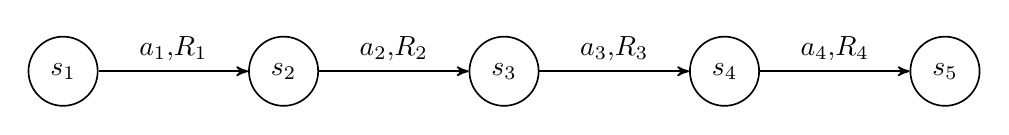
\begin{tikzpicture}[->,>=stealth',auto,node distance=2.8cm,semithick]
\tikzstyle{every state}=[text=black]
\node[state]         (s1)					{$s_1$};
\node[state]         (s2) [right of=s1] {$s_2$};
\node[state]         (s3) [right of=s2] {$s_3$};
\node[state]         (s4) [right of=s3] {$s_4$};
\node[state]         (s5) [right of=s4] {$s_5$};


\path	(s1) edge node		 {$a_1$,$R_1$} (s2)
		 (s2) edge node		 {$a_2$,$R_2$} (s3)
		 (s3) edge node		 {$a_3$,$R_3$} (s4)
		 (s4) edge node		 {$a_4$,$R_4$} (s5);

\end{tikzpicture}\\
\\
Now lets formulate eligibility for each of the $5$ states for $5$
time steps.\\
\\

\begin{tabular}{|c|c|c|c|c|c|}
\hline 
$E_{i}(s_{j})$ & $s_{1}$ & $s_{2}$ & $s_{3}$ & $s_{4}$ & $s_{5}$\tabularnewline
\hline 
\hline 
$e_{0}$ & $0$ & $0$ & $0$ & $0$ & $0$\tabularnewline
\hline 
$e_{1}$ & $1$ & $0$ & $0$ & $0$ & $0$\tabularnewline
\hline 
$e_{2}$ & $\gamma\lambda$ & $1$ & $0$ & $0$ & $0$\tabularnewline
\hline 
$e_{3}$ & $(\gamma\lambda)^{2}$ & $\gamma\lambda$ & $1$ & $0$ & $0$\tabularnewline
\hline 
$e_{4}$ & $(\gamma\lambda)^{3}$ & $(\gamma\lambda)^{2}$ & $\gamma\lambda$ & $1$ & $0$\tabularnewline
\hline 
$e_{5}$ & \textbf{$0$} & $(\gamma\lambda)^{3}$ & $(\gamma\lambda)^{2}$ & $\gamma\lambda$ & $1$\tabularnewline
\hline 
\end{tabular}\\
\\
Now let $V$ denote the value function estimate for all the states
as a vector i.e $V_{i}=V(s_{i})$. When we do online updates to $V$
using eligibility traces, say $V(s_{1})$ - will get updated till
time epoch $4$ as its eligibility goes to $0$ after that. Also,
we are assuming that $s_{1}$ is not visited till its eligibility
goes to $0$ ( This is not necessary, but makes the proof simple :)
). So let us consider the total reward which is used to update $V(s_{1})$.\\
\\
\begin{alignat*}{1}
V & \leftarrow V+\alpha\delta e^{(t)}
\end{alignat*}
 where $e^{(t)}$ denotes eligibility vector ( for all states ) at
time instant $t$.\\
\\
Now for $V(s_{1})$, the updates are as follows.\\
\\
\begin{alignat*}{1}
V(s_{1}) & \leftarrow V(s_{1})+\alpha\{R_{1}+\gamma V(s_{2})-V(s_{1})+\gamma\lambda\{R_{2}+\gamma V(s_{3})-V(s_{2})\}+(\gamma\lambda)^{2}\{R_{3}+\gamma V(s_{4})-V(s_{3})\}\\
 & +(\gamma\lambda)^{3}\{R_{4}+\gamma V(s_{5})-V(s_{4})\}\}
\end{alignat*}
\\
Now this big summation can be reduced by simple math manipulations.
Lets decompose,

\begin{alignat*}{1}
R_{1} & =R_{1}(1-\lambda)+R_{1}(1-\lambda)\lambda+R_{1}(1-\lambda)\lambda^{2}+R_{1}(1-\lambda)\lambda^{3}+R_{1}\lambda^{4}
\end{alignat*}

\begin{alignat*}{1}
R_{2} & =R_{2}(1-\lambda)+R_{2}(1-\lambda)\lambda+R_{2}(1-\lambda)\lambda^{2}+R_{2}\lambda^{3}
\end{alignat*}

\begin{alignat*}{1}
R_{3} & =R_{3}(1-\lambda)+R_{3}(1-\lambda)\lambda+R_{3}\lambda^{2}
\end{alignat*}
\\
So the above expression can be rewritten as given below.\\
\\
$V(s_{1})\leftarrow V(s_{1})+\alpha\{(1-\lambda)\{\{\lambda^{0}\{R_{1}+\gamma V(s_{2})\}+\lambda^{1}\{R_{1}+\gamma R_{2}+\gamma^{2}V(s_{3})\}+\lambda^{2}\{R_{1}+\gamma R_{2}+\gamma^{2}R_{3}+\gamma^{3}V(s_{4})\}+\lambda^{3}\{R_{1}+\gamma R_{2}+\gamma^{2}R_{3}+\gamma^{3}R_{4}+\gamma^{4}V(s_{5})\}\}+\lambda^{4}\{R_{1}+\gamma R_{2}+\gamma^{2}R_{3}+\gamma^{3}R_{4}+\gamma^{4}V(s_{5})\}\}-V(s_{1})\}$\\
\\
i.e $G^{\lambda-eff}=$ $\sum_{i=1}^{4}\lambda^{i-1}G^{(i)}+\lambda^{4}G^{(4)}$
where $G^{(i)}=i-step\,TD\,return.$

\subsection{Part (b)}

From the above analysis, we can generalise it to $(\gamma\lambda)^{n}$
truncation case ( after $n$ time steps ).

$G^{\lambda-eff}=$ $\sum_{i=1}^{n+1}\lambda^{i-1}G^{(i)}+\lambda^{n+1}G^{(n+1)}$
where $G^{(i)}=i-step\,TD\,return$.

\section{Problem 5}

A Markov state provides complete information which is required for
making decisions from the particular state. It can be some representation
of the history of all the past states, actions and rewards. It need
not contain all the details about the history but will contain information
which is essential for future decisions. In other words, best policy
obtained using Markov states is as good as the one which we obtain,
if we use complete histories. Using this idea, lets see what happens
in the Broken vision system problem.\\
\\
When we see the first scene, we just see a portion of the environment
- just a single snapshot. We can't see what is behind us? We can't
see occluded objects? In this case, we can say that we have access
to a Markov state if suppose we know the rules of the environment
dynamics. This is because if the environment operates based on some
set of rules and the maximum information which we can get from the
environment is: the first scene, we do have access to a Markov state.
It contains information based on which all future decisions can be
taken.\\
\\
On the other hand, if the camera is broken we won't have images of
the environment. These images might prove crucial to a future decision
which we might take, and we are missing that! So, in this case we
don't have access to a Markov state as we might not have all the required
information needed to make a decision in the future.

\section{Problem 6}

Q-learning is an off-policy method and using it, we can learn optimal
policies even if we follow random exploratory policies to generate
episodes. Similarly, if we use on-policy methods, we need to use importance
sampling if the behaviour policy and target policy are different.\\
\\
Now suppose we have the optimal policy in hand. We need to learn the
value function of an arbitrary policy while following the optimal
policy. To learn the value function of an arbitrary policy ( not optimal
) we need to use some on-policy method say SARSA. And we need to generate
trajectories from that policy. Since, we are using the optimal policy
to generate trajectories we can use importance sampling to weigh the
updates and hence make sure that the estimated Q-values correspond
to the arbitrary policy.\\
\\
But this method has a higher variance and you can reduce it a bit
using Weighted importance sampling at the cost of added bias. Another
important thing to ensure is that the optimal policy should cover
the arbitrary policy i.e it should be stochastic in places wherever
the arbitrary policy is stochastic. This is important otherwise the
weight blows to $\infty$.

\section{Problem 7}

The bhajji vendor's business depends on a variety of factors. All
he can do is to buy raw materials or make bhajjis and sell them. His
goal is to get maximum profit inspite of the stochasticity involved
in this problem.\\
\\
In RL terms, all these factors constitute the ``state'' of the vendor.
It will contain all information which will be required to take future
decisions. The ``actions'' which can be taken by the vendor are
- \{ buy raw materials, sell bhajjis \}. Now the ``reward'' which
the vendor gets - should be such that we get an optimal policy considering
the dependencies on all the factors.\\
\\
The state representation contains: $\begin{array}{c}
last\,delivery\,time\,for\,all\,raw\,materials\,(for\,previous\,order)\,[tod_{last}]\\
whether\,end\,sem\,exams\,are\,going\,on\,in\,IIT\,[is\_exam\_going\_on]\\
expiry\,date\,for\,all\,raw\,materials\,[toe]\\
current\,quantities\,of\,raw\,materials\,[Q_{r}]
\end{array}$\\
\\
The action-set is: $\{buy\,raw\,materials\,from\,a\,particular\,vendor,sell\,bhajjis\}$.
Note that the state gets changed when an action is taken - learnt
using simulation. That's where RL comes into play.\\
\\
All penalties or positive feedback are provided through rewards. The
reward function should consider the following factors into account:
profit which he gets ( depends on number of bhajjis sold, selling
price, cost price and the holding price - depends on current time
and last time of delivery of raw materials ), penalty imposed based
on current time, time of last delivery and expiry date. The profit
term takes care of the under-ordering problem whereas the penalty
term takes care of the over-ordering problem. So, a possible expression
for reward is:\\
\\
\begin{alignat*}{1}
R & =\lambda(s.p-c.p-H(t-tod_{last}))+max(t-tod_{last},toe-tod_{last})
\end{alignat*}
\\
\\
where $\lambda$ is a hyperparameter, $s.p$ denotes selling price,
$c.p$ denotes cost price and $H$ denotes the holding cost per unit
time.\\
\\
Based on the above formulation if we sample transitions from various
episodes ( based on the data collected by him ), we can find the optimal
policy - which gives the action to take in the current state. Thus,
the given problem can be solved using RL.

\section{Problem 8}

\subsection{Part (a)}

Return $G_{t}=R_{t+1}+R_{t+2}+R_{t+3}+...+R_{t+k}$.\\
\\
No. The above return doesn't result in an optimal policy. Optimality
equation is defined

\section{Problem 9}

The proof of Bellman Optimality equation involves usage of Banach
fixed point theorem and triangle inequality. To use Banach fixed point
theorem, we need to prove that the transformation $L=max_{a}\{r(s,a)+\gamma p(j|s,a)V(j)\}$
is a contraction. This transformation is a contraction only when $\gamma<1$.
So if $\gamma=1$, this transformation will not be a contraction and
as a result Banach fixed point theorem cannot be applied. This means
that, the proof of convergence doesn't hold when $\gamma=1$.\\
\\
When we go through the proof of convergence of Bellman optimality
equation, we will find that the bound used for proving that $L$ is
a contraction is a very loose bound.\\
\\
\begin{alignat*}{1}
|LV(s)-LU(s)| & \leq\gamma\sum_{j}P(j|s,a_{s}^{*})(V(j)-U(j))
\end{alignat*}
\\
The above expression gets reduced to,\\
\\
\begin{alignat*}{1}
|LV(s)-LU(s)| & \leq\sum_{j}P(j|s,a_{s}^{*})(V(j)-U(j))
\end{alignat*}

\begin{alignat*}{1}
|LV(s)-LU(s)| & \leq||V-U||\{\sum_{j}P(j|s,a_{s}^{*})\}
\end{alignat*}

\begin{alignat*}{1}
|LV(s)-LU(s)| & \leq||V-U||
\end{alignat*}
Note that $||..||$ is max-norm and the bound used in the above step
is a very loose bound. As a result, we still maintain the equality
sign and there is no contracting factor in the expression. If we use
an alternative way to bound this and hence obtain a way to prove,\\
\\
\begin{alignat*}{1}
||LV-LU|| & <\lambda||V-U||
\end{alignat*}
\\
\\
where $0\leq\lambda<1$, then we can prove that $L$ is a contraction
which means Banach fixed point theorem will hold and hence there is
a unique fixed point to Bellman optimality equation. Thus, it will
guarantee the existence of a unique solution.

\section{Problem 10}

Many real world problems have a large number of states and hence traditional
DP methods fail due to memory/time constraints. So we resort to methods
like Realtime dynamic programming which obtains better estimates for
the states which are more frequently visited. But the algorithm can
be improved if we exploit the symmetries involved in the problem.
Similar states tend to have similar optimal actions and hence number
of computations can be minimised if these symmetries are used while
solving the MDP.\\
\\
Since the accuracy of estimates depends on the number of samples which
was used to estimate them, our goal is to determine the sampling strategy
based on symmetries so that it performs better than existing RTDP
algorithm, when we have state-spaces with symmetries.

\subsection*{Algorithm}

\section{Problem 11}

We have a bandit problem in which the parameters on which the policy
depends are the preferences of the actions and the action selection
probabilities are determined using a softmax relationship as:

\begin{alignat*}{1}
\pi_{t}(a_{j})= & \frac{e^{p_{t}(a_{j})}}{\sum_{i=1}^{n}e^{p_{t}(a_{i})}}
\end{alignat*}
\\
where $p_{t}(a)$ is the preference of action $a$ at time $t$.\\
\\
The REINFORCE update equation is:\\
\\
\begin{alignat*}{1}
\theta_{t+1} & \leftarrow\theta_{t}+\alpha_{t}(r_{t}-b_{t})\nabla_{p_{t}}log(\pi_{t}(a_{t}))\frac{\partial p_{t}}{\partial\theta_{t}}
\end{alignat*}
$ $\\
where baseline $b_{t}$ is defined as $b_{t+1}=b_{t}+\beta(r_{t}-b_{t})$.\\
\\
Solving we get,

\begin{alignat*}{1}
\theta_{t+1} & \leftarrow\theta_{t}+\alpha_{t}(r_{t}-b_{t})\{1-\pi_{t}(a_{t})\}\frac{\partial p_{t}}{\partial\theta_{t}}
\end{alignat*}


\section{Problem 12}

Let us consider a Gaussian parameterization for the same. Parameters
are mean $\mu$ and variance $\sigma^{2}$ of the Normal distribution
and baseline $b_{t}=0$.\\
\\
\begin{alignat*}{1}
\pi_{t}(a;\mu_{t},\sigma_{t})= & \frac{1}{\sqrt{2\pi\sigma}}e^{-\frac{(a-\mu_{t})^{2}}{\sigma_{t}^{2}}}
\end{alignat*}
\\
\\
The REINFORCE update equation is:\\
\\
\begin{alignat*}{1}
\theta_{t+1} & \leftarrow\theta_{t}+\alpha_{t}(r_{t}-b_{t})\nabla_{\theta_{t}}log(\pi_{t}(a_{t}))
\end{alignat*}
\\
\\
Here $\theta_{t}=\begin{array}{c}
\mu_{t}\\
\sigma_{t}
\end{array}$ . Solving we get,\\
\\
\begin{alignat*}{1}
\mu_{t+1} & \leftarrow\mu_{t}+\alpha_{t}r_{t}(a_{t}-\mu_{t})
\end{alignat*}
\\
\\
\begin{alignat*}{1}
\sigma_{t+1} & \leftarrow\sigma_{t}+\frac{\alpha_{t}r_{t}\{(a_{t}-\mu_{t})^{2}-\sigma_{t}^{2}\}}{\sigma_{t}}
\end{alignat*}

\end{document}
